\chapter{Heteroskedasticity}
\label{sec:het}
Recall the typical regression model
\[
y_i=\beta_0+\sum_p\beta_px_{ip}+e_i
\]
We make the assumption that
\[
\mbox{var}\left(e_i\right)=\sigma^2
\]
Note how there is no subscript on sigma squared. We assume that the variance is constant for each case $i$. That is, we assume {\it \underline{homo}skedasticity}. We can visualize homoskedasticity in Figure~\ref{fig:hetokcurv}, where the residuals of each prediction have a relatively constant distribution.

{\it \underline{Hetero}skedasticity}, where $\sigma^2$ is not constant across values of our predictions, can cause standard errors to be biased, making hypothesis tests difficult to interpret. We can visualize heteroskedasticity in Figure~\ref{fig:hetnotokcurv}, where the residuals of each prediction are not consistent.

\begin{figure}
   \centering
   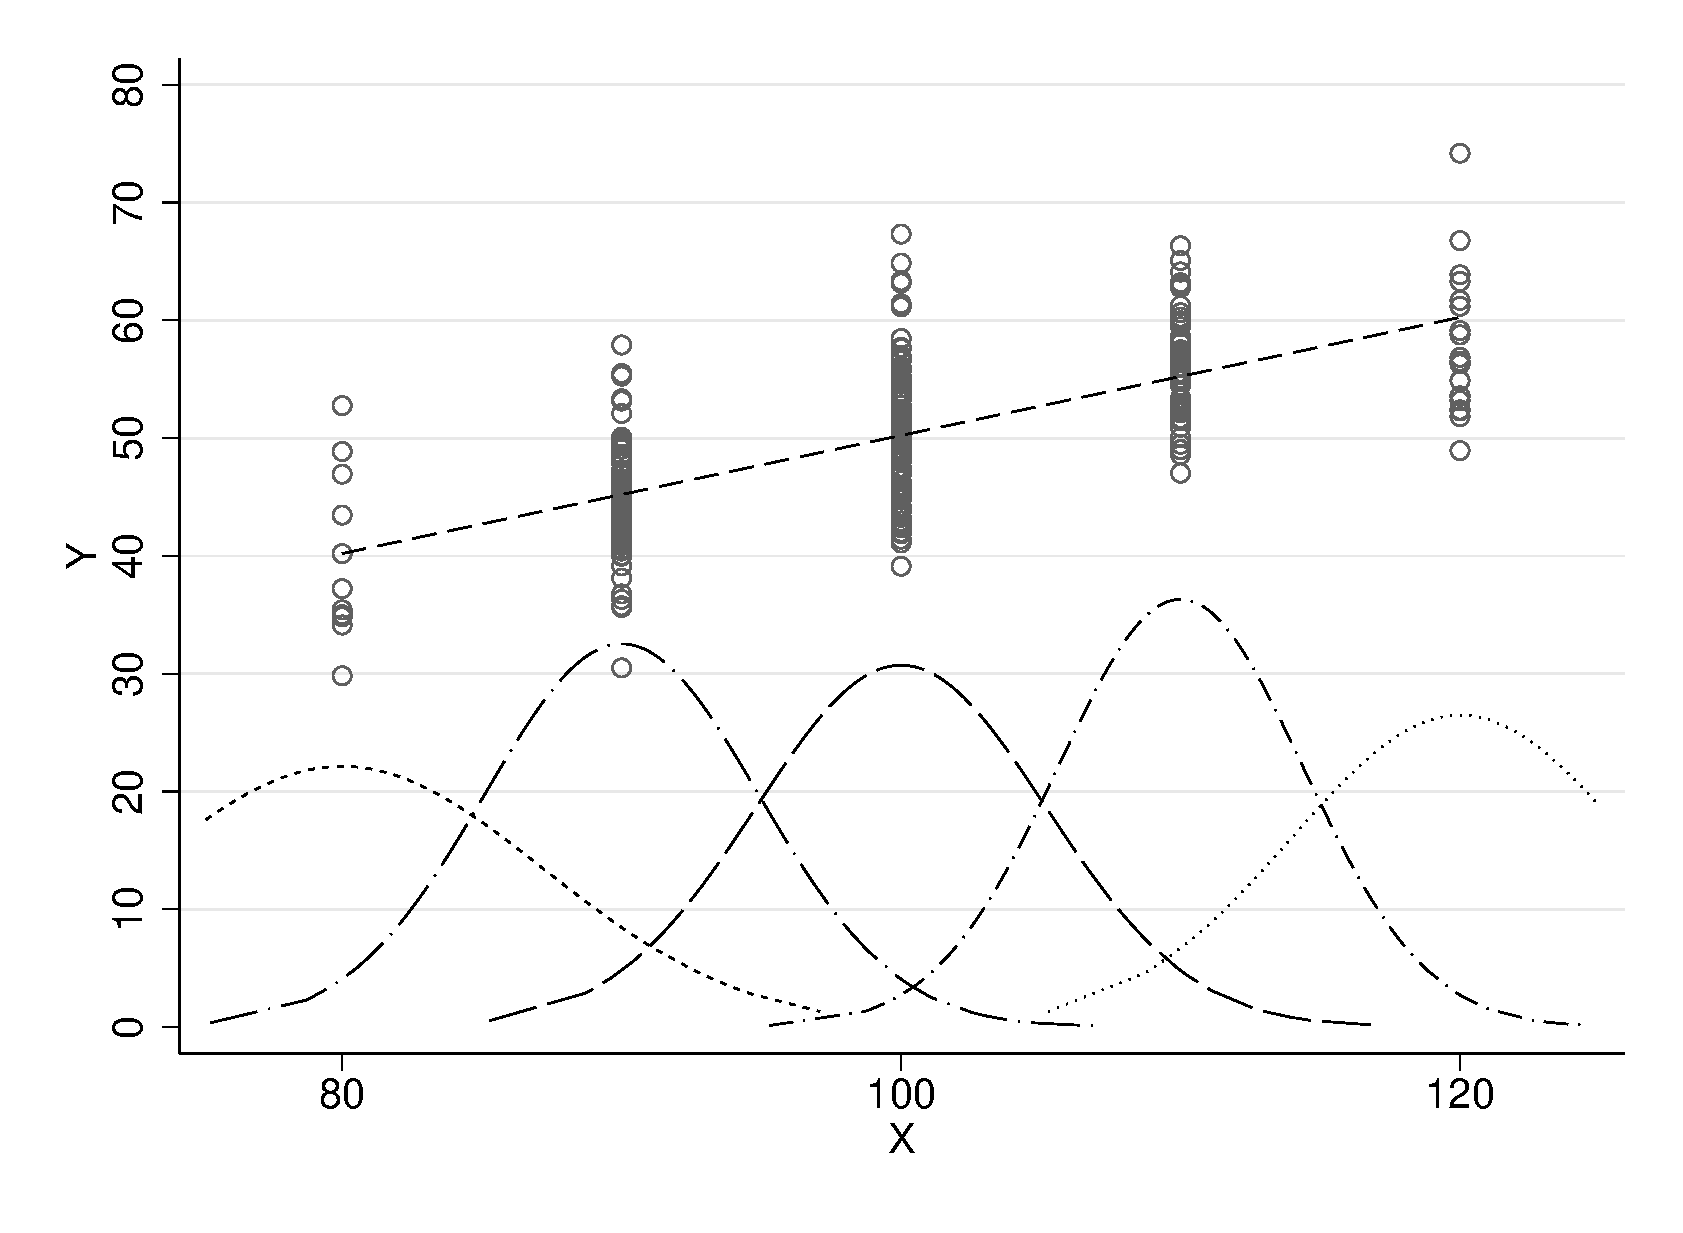
\includegraphics[angle=0,
           width=.75\textwidth]{hetokcurv.eps}
   \caption{Regression with relatively constant variance}
  \label{fig:hetokcurv}
\end{figure}
\begin{figure}
   \centering
   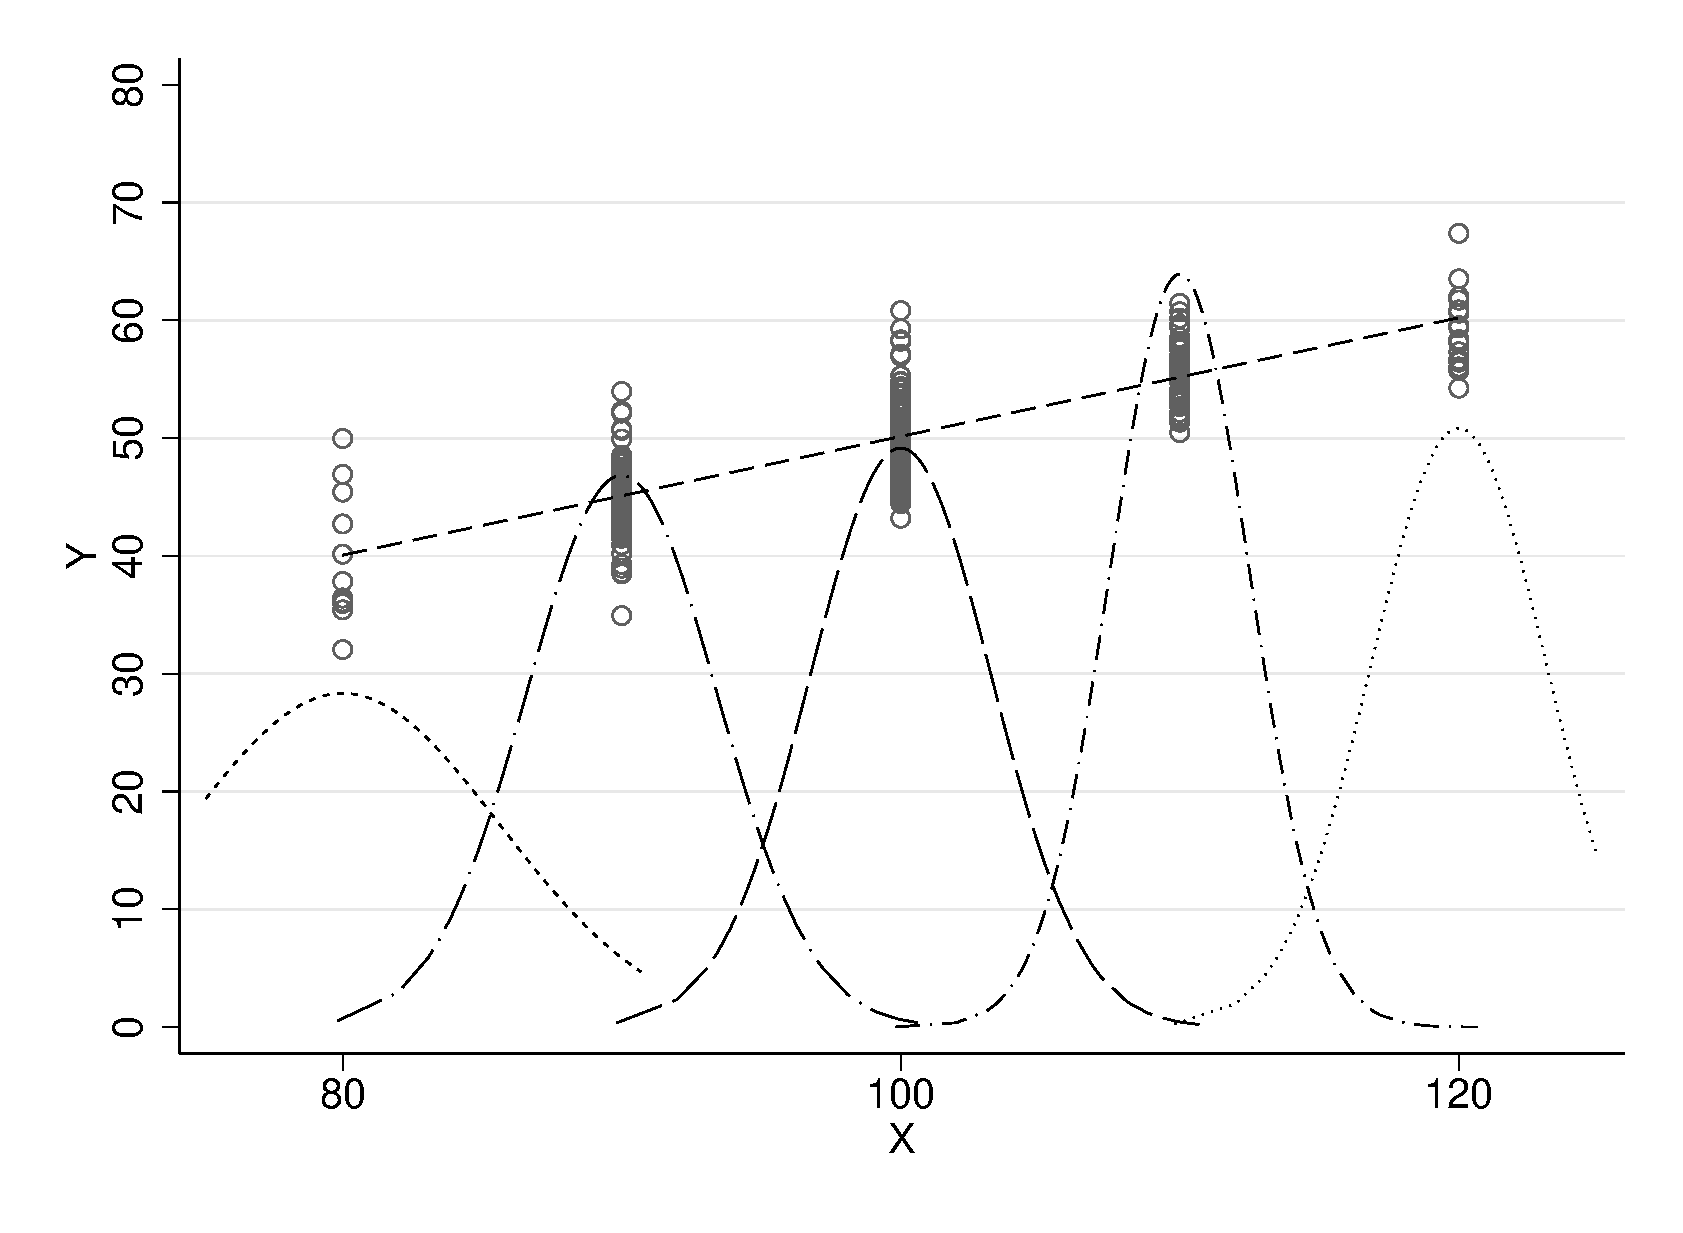
\includegraphics[angle=0,
           width=.75\textwidth]{hetnotokcurv.eps}
   \caption{Regression with non-constant variance}
  \label{fig:hetnotokcurv}
\end{figure}

\section{Why non-constant variance is a problem}

In bivariate regression, we can represent the variance (the square of the standard error) of the slope as equation~\eqref{eq:olsb1var}
\[
\mbox{var}\left(\beta_1\right)=\frac{\sigma^2}{\sum_{i=1}^N\left(x_i-\bar{x}\right)^2}
\]
where $\sigma^2$ is the variance of the residuals. Mechanically, it just means that the standard error is a function of the variance of the residuals standardized by the sum of squares in the predictor.

We do not actually know the true variance of the residuals, so we estimate the variance of the residuals with
\begin{equation}
\hat{\sigma}^2=\frac{\sum_{i=1}^N\hat{e}_i^2}{N-p}
\end{equation}
and assume that it is constant for all predicted values, $\hat{y}_i$. When the variance of the residuals is not constant, then the formula for the variance of the slope is more complicated
\begin{equation}
\mbox{var}\left(\beta_1\right)=\frac{\sum_{i=1}^N\left(\left(x_i-\bar{x}\right)^2\sigma_i^2\right)}{\left(\sum_{i=1}^N\left(x_i-\bar{x}\right)^2\right)^2}
\end{equation}
Now, the variance of the residual is unique for each case (note the subscript $i$ on $\sigma_i^2$) and is scaled by the squared deviation from the mean. We a critical problem: since we only have one observation for each prediction, there is no way to estimate the variance of the errors for that prediction. OLS regression software does not know this, so estimates of the standard errors are potentially biased.

The direction of this bias is not consistently reported in statistical texts. Econometricians generally think that the variances are overestimated, leading to difficulty in rejecting hypotheses. This would be annoying, but somewhat acceptable with large samples. However, others believe that the direction of the bias is unknown, so in some cases the null hypothesis rejection is false.

\section{Testing for heteroskedasticity}

When the issue is introduced, often people show a figure like Figure~\ref{fig:hetero}. However, it often doesn't look this straightforward. More often, you need theory to tell you that you should expect heteroskedastic relationships and you should plan ahead for them.  We again return to charity and household income; see Tables~\ref{tab:charitydes} and \ref{tab:charity} in the discussion of logs in \ref{sec:logs}.

We expect that the variance of giving is going to be lower for lower-income households (they just do not have as much) and higher for richer households (some give, some do not, some give a lot). We can examine a regression of charity on income, visually, and inspect a plot of the residuals by the prediction, $\hat{y}_i$. I do this in Figure~\ref{fig:hetcharity}. Notice how the "spread" of residuals differs based on the prediction.

\begin{figure}
   \centering
   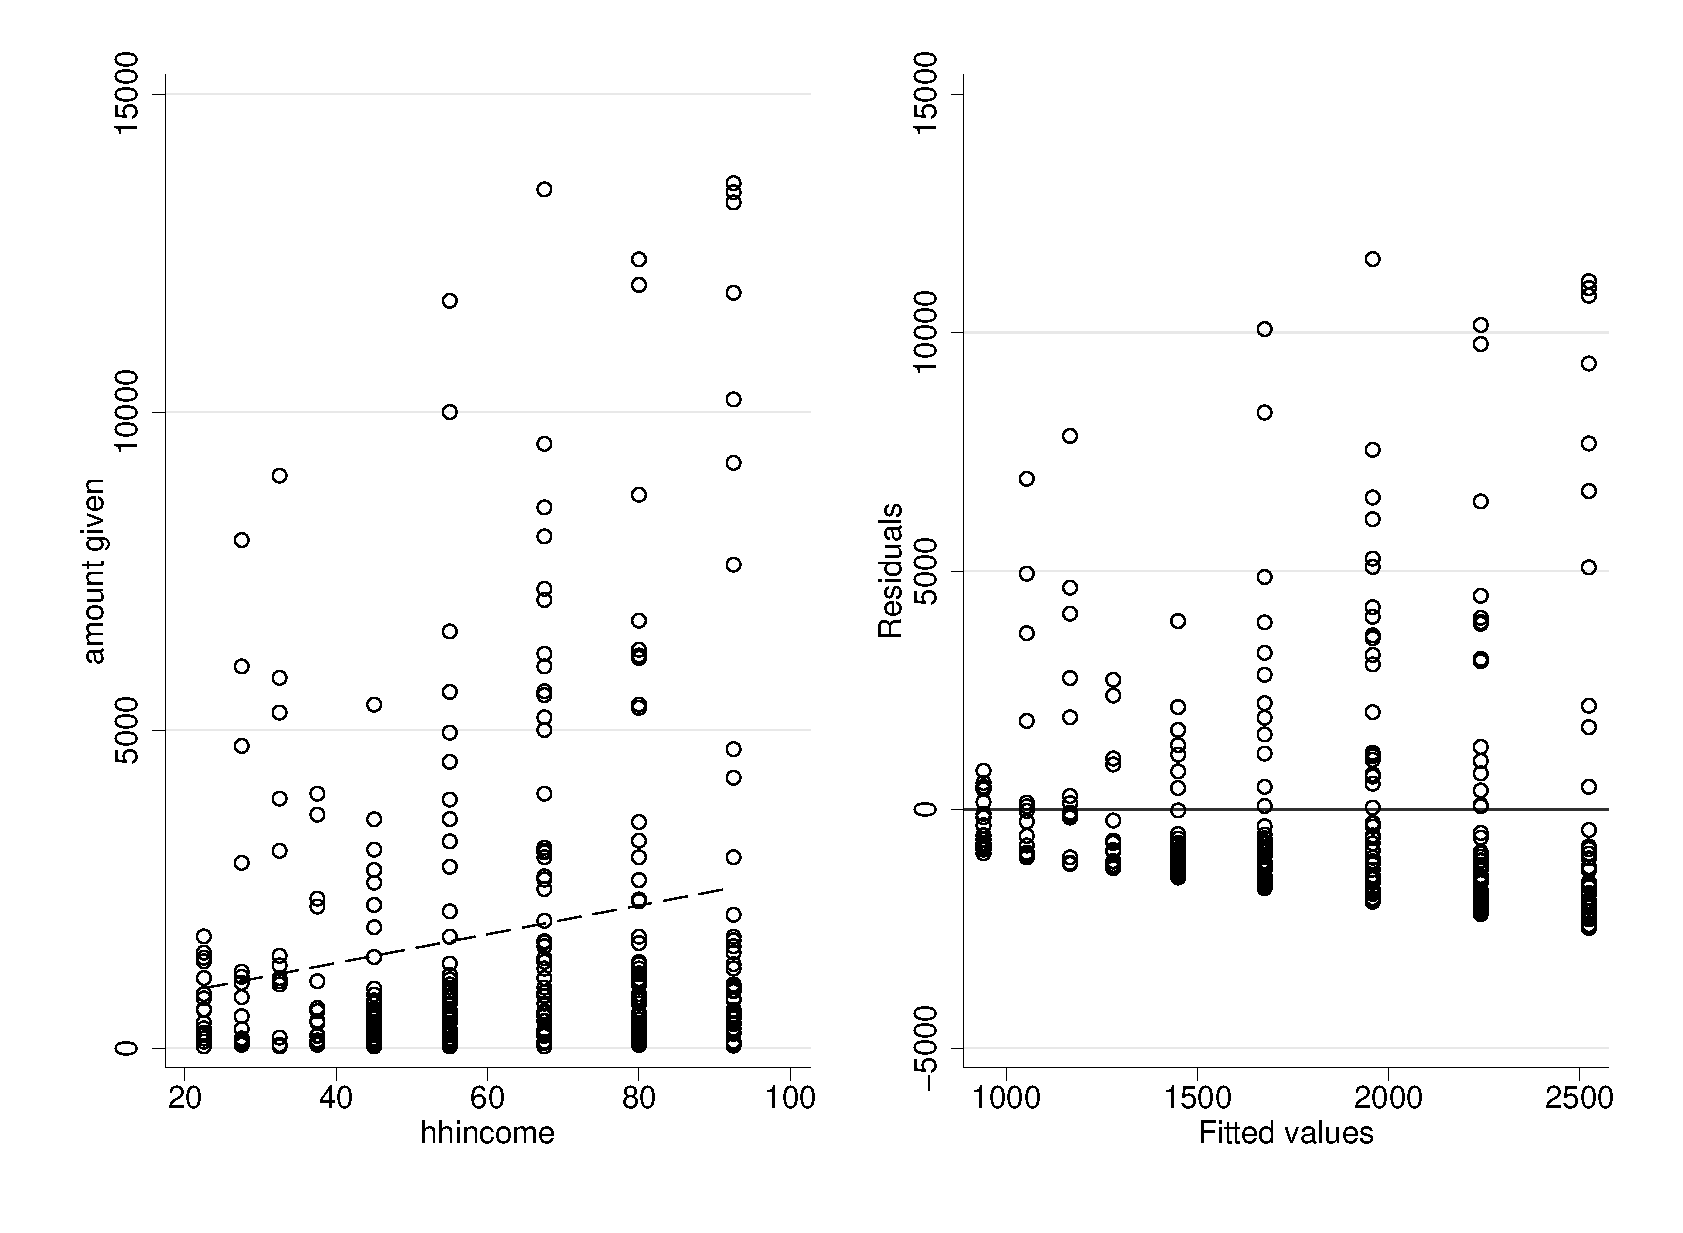
\includegraphics[angle=0,
           width=.75\textwidth]{hetcharity.eps}
   \caption{Regression of charity on income (left), residuals by fitted values (right)}
  \label{fig:hetcharity}
\end{figure}

How can we detect heterskedasticity without having to look at graphics?

One simple test is called the Breusch-Pagan test. It tests for a function to the variance of the residuals based on a set of predictors. The logic of the test is that if there is heteroskedasticity, then the magnitude of the residuals (and thus the variance) would be dependent on some set of predictors. In other words, if we have a regression model
\[
y_i = \beta_0+\beta_1x_i+e_i
\]
we then suppose some variance function
\[
\frac{e_i^2}{\sigma^2}=\gamma_0+\gamma_1z_{1i}\ldots\gamma_kz_{ki}+v_i
\]
Where $e_i$ is the residual of each case and $\sigma^2$ is the variance of all the residuals. The reason for the denominator is to standardize the residuals to a z-score, which makes the results of the test applicable to a $\chi^2$ distribution. If it is not immediately obvious how this standardization occurs, recall that a $z$-score takes the form of
\[
z_i = \frac{x_i-\bar{x}}{s}
\]
where the numerator, $x_i-\bar{x}$, is the difference between an observed case and the mean and the denominator, $s$, is the standard deviation. Now consider that a residual is just the difference between an observed case and the predicted value, $e_i=y_i-\hat{y}$, that has a mean of 0.

Since a predicted value is just a conditional mean, we can see the analogue to a $z$-score numerator. In this notation, we consider $\sigma^2$ to be the variance of the residuals. Therefore, $\sigma$ is the standard deviation of the residuals. With all of these pieces, we can see that the dependent variable of our variance function, $\frac{e_i^2}{\sigma^2}$, is basically a $z$-score.

By default, we use the predicted values of $y$ as our predictor for the variance function. This is a convenient thing to do when we have several predictors since $\hat{y}$ is just a linear combination of the predictors anyway.

The test procedure is this. Suppose we fit a model to the data
\[
y_i = \beta_0+\sum_p\beta_px_{pi}+e_i
\]
and predicted the fitted values
\[
\hat{y}_i = \beta_0+\sum_p\beta_px_{pi}
\]
and estimated the variance of the residuals, $\hat{\sigma}^2$, using the models sum of squared errors, $SSE_{model}$:
\begin{equation}
\hat{\sigma}^2=\frac{SSE_{model}}{N}
\end{equation}
We then calculate a standardized residual
\begin{equation}
u_i=\frac{e_i^2}{\hat{\sigma}^2}
\end{equation}
and fit an auxiliary model using the fitted values as a predictor
\[
u_i=\gamma_0+\gamma_1\hat{y}_i+v_i
\]
We then find the sum of squares regression for this auxiliary regression model ($SSR_{auxiliary}$) and divide it by 2:
\begin{equation}
\theta=\frac{SSR_{auxiliary}}{2}
\end{equation}
This statistic has a $\chi^2$ distribution with 1 degree of freedom. Thus, it can be statistically evaluated. If this statistic is greater than about 3.84, then the model is likely heterskedastic.

The logic is that if the sum of squares for the regression in this auxiliary model is large, then there is a relationship between the {\it magnitude} of the residual and the predictor(s) of the original model.

\subsection{Breusch-Pagan example}

For example, Model 1 in Table~\ref{tab:charityhet} produced a set of residuals that were converted in a standardized outcome. The auxiliary model produced a sum of squares regression of 85.570, see Table~\ref{tab:charityresid}. We then calculate our test
\[
\theta=\frac{SSR_{auxiliary}}{2}=\frac{85.570}{2}=42.785
\]
Which has a $p$-value of 0.00000000003; statistically significant.

This is a problem for the analysis as it is. While the point estimates (the slope) are trustworthy, the standard errors are not (they may be too big, they may be too small) making hypothesis testing difficult. The rest of this chapter is devoted to what you can do to generate appropriate standard errors while essentially preserving the model.

\section{Robust standard errors}

The first method to combat heterskedasticity is to directly address the standard errors. Thus, we want to estimate robust standard errors. Recall the issue is that with non-constant variance, the variance estimate of the bivariate slope is
\begin{equation}
\mbox{var}\left(\beta_1\right)=\frac{\sum_{i=1}^N\left(\left(x_i-\bar{x}\right)^2\sigma_i^2\right)}{\left(\sum_{i=1}^N\left(x_i-\bar{x}\right)^2\right)^2}
\end{equation}
Recall that the problem was that there was no way to estimate the variance of a single residual $\sigma_i^2$. However, Hal White suggested that we substitute with each case's squared residual instead to produce
\begin{equation}
\mbox{var}\left(\beta_1\right)=\frac{\sum_{i=1}^N\left(\left(x_i-\bar{x}\right)^2e_i^2\right)}{\left(\sum_{i=1}^N\left(x_i-\bar{x}\right)^2\right)^2}
\end{equation}
Why would $e_i^2$ make a good substitute for $\sigma_i^2$? Remember that a population variance is the sum of squared deviations from the mean divided by the number in the population
\[
\mbox{var}\left(x\right)=\frac{\sum_{i=1}^N\left(x_i-\bar{x}\right)^2}{N}
\]
Since the expected mean residual is 0, and we only have 1 observation,
\[
\mbox{var}\left(e\right)=\frac{\sum_{i=1}^1\left(e_i-0\right)^2}{1}=\frac{\sum_{i=1}^1\left(e_i\right)^2}{1}=e_i^2
\]
Thus, the square of the residual is a good choice. All robust standard errors do is fit the original model, save the residuals, and reuse them to calculate new variances. Model 2 in Table~\ref{tab:charityhet} presents robust standard errors. Note that in this case, the standard error of the slope is larger.

\subsection{Robust standard errors in matrix notation}
\label{sec:robustmatrix}
Recall from \ref{sec:matrixv} that the variance of the slopes is expressed as
\[
\bf V\left({\hat{b}}\right)=\left(\frac{1}{N}X'X\right)^{-1}\sigma^2
\]
This expression also makes the assumption of constant variance. The expression is more complicated in its general form without this assumption
\begin{equation}
\bf V\left({\hat{b}}\right)=\left(X'X\right)^{-1}X'\left(V\left(y\right)\right)X\left(X'X\right)^{-1}
\end{equation}
When we assume constant variance and uncorrelated errors, then
\begin{equation}
\bf V\left(y\right)=\sigma^2 \it I
\end{equation}
Where $\bf \it I$ is a matrix of 1s in the diagonal and 0s otherwise. For example, if we had 4 observations, then
\[
\bf \it I =
\begin{bmatrix}
1&0&0&0 \\
0&1&0&0 \\
0&0&1&0 \\
0&0&0&1 \\
\end{bmatrix}
\]
When we multiply this matrix by the scalar such as $\sigma^2$, then the diagonals become $\sigma^2$ and the off diagonals stay 0:
\[
\bf \sigma^2\it I =
\begin{bmatrix}
\sigma^2&0&0&0 \\
0&\sigma^2&0&0 \\
0&0&\sigma^2&0 \\
0&0&0&\sigma^2 \\
\end{bmatrix}
\]
This all makes $\bf V\left(y\right)$ a very simple entity of the same scalar along the diagonals, allowing us to cancel out most of the $\bf X'X$s. This leaves us with $\bf \sigma^2\left(X'X\right)$ to express the variances of our slopes. However, when we have non-constant variances then we are no longer dealing with a single scalar. Instead, we theoretically have a variance for each case, $\sigma_i^2$. This makes
\begin{equation}
\bf V\left(y\right)=\mbox{diag}\left\{\sigma_1^2\ldots\sigma_N^2\right\}
\end{equation}
The "diag" notation is a short hand for saying the following elements are along the diagonal on a matrix that is otherwise 0s. For example, in our 4 case scenario,
\[
\bf V\left(y\right) =
\begin{bmatrix}
\sigma_1^2&0&0&0 \\
0&\sigma_2^2&0&0 \\
0&0&\sigma_3^2&0 \\
0&0&0&\sigma_4^2 \\
\end{bmatrix}
\]
Of course, as we noted before, we do not know $\sigma_i^2$. Instead, as White suggested, we define a matrix where the diagonal is the square of the residuals
\begin{equation}
\bf \Sigma=\mbox{diag}\left\{e_1^2\ldots e_N^2\right\}
\end{equation}
We then use that for our variance estimation
\begin{equation}
\bf V\left(b_{robust}\right)=\left(X'X\right)^{-1}X'\Sigma X\left(X'X\right)^{-1}
\end{equation}
This is often called a "sandwich" estimator because we sandwich $\Sigma$ in between two instances of $\bf \left(X'X\right)^{-1}$.

\section{Generalized least squares}
\label{sec:glmintro}

The second approach to addressing heterskedasticity is to address the variance function directly. In this case, we theorize that the magnitude of the residuals, and thus the variance of them, is correlated with $x$. For our example, we believe that the variance of giving to charity increases with household income. Thus, we can weight the data in such a way to compensate for this relationship.

We can estimate our models by way of weighted least squares (WLS) and take two approaches to doing so: (a) we can assume we "know" a simple relationship between our errors and a predictor or (b) we can estimate the variance function to make a feasible model.

\subsection{Weighted least squares}

One possible way to think about this relationship is that the observed variance for a residual is a function of the "true" variance proportional to the magnitude of our predictor
\[
\mbox{var}\left(e_i\right)=\sigma^2x_i
\]
Following White's suggestion that the best guess of the variance of a single residual is the square of the residual, we can easily see that our observed residuals, , are a product of the true residual and the square root of $x$
\begin{equation}
e_i^2=u_i^2x_i
\end{equation}
\[
e_i=u_i\sqrt{x_i}
\]
\[
\frac{e_i}{\sqrt{x_i}}=u_i
\]
Thus, the only logical thing to do to estimate the true error, $u_i$, is to divide the entire model (including the intercept) by $\sqrt{x_i}$
\begin{equation}
\frac{y_i}{\sqrt{x_i}}=\beta_0\frac{1}{\sqrt{x_i}}+\beta_1\frac{x_i}{\sqrt{x_i}}+\frac{e_i}{\sqrt{x_i}}
\end{equation}
In effect, this procedure weights the data by
\begin{equation}
w_i=\frac{1}{\sqrt{x_i}}
\end{equation}
The results of this model are presented as Model 3 in Table~\ref{tab:charityhet}.

\subsection{Weighted least squares in matrix form}

We again return to matrix algebra to see how this generalizes to the least squares linear model. If we make the strong assumption that variances of the errors are proportional to another variable like $\sigma_i^2=\sigma^2/w_i^2$, then we know that the likelihood of the model is
\begin{equation}
L\left({\bf b},\sigma^2\right)=\frac{1}{\left(2\pi\right)^{\frac{N}{2}}}e^{\left(-\frac{1}{2}\bf{\left(y-Xb\right)'\Sigma^{-1}\left(y-Xb\right)}\right)}
\end{equation}
where
\begin{equation}
\Sigma = \sigma^2\times \mbox{diag}\left\{\frac{1}{a_i^2}\ldots\frac{1}{w_N^2}\right\}={\bf \sigma^2W^{-1}}
\end{equation}
With this likelihood function we can get to the formula for the coefficients that maximizes the likelihood and minimizes the squares of the weighted errors, $\sum_{i=1}^N\left(w_ie_i\right)^2$
\begin{equation}
\bf b_{WLS}=\left(X'WX\right)^{-1}X'Wy
\end{equation}
where
\begin{equation}
{\bf W} = \mbox{diag}\left\{w_1\ldots w_N\right\}
\end{equation}
Compare this the OLS estimator,~\eqref{eq:olsmatrix}
\[
{\bf{b=\left(X'X\right)^{-1}X'y}}
\]
It is almost the same thing except that the weight matrix is sandwiched in there. The variance-covariance matrix of these slopes is
\begin{equation}
\bf V\left(b_{WLS}\right)=\sigma^2\left(X'WX\right)^{-1}
\end{equation}
Compare this to the OLS variances
\begin{equation}
\bf V\left(b_{OLS}\right)=\sigma^2\left(X'X\right)^{-1}
\end{equation}
Again, it is almost the same thing except for the addition of the weight matrix. However, you may wish to use the robust-weighted variances, which like White's robust variances is a somewhat complicated expression
\begin{equation}
\bf V\left(b_{WLS, robust}\right)=\left(X'WX\right)^{-1}X'W\Sigma WX\left(X'WX\right)^{-1}
\end{equation}
However, you should be able to see the resemblance to the typical robust errors we just covered in \ref{sec:robustmatrix}.
\begin{equation}
\bf V\left(b_{robust}\right)=\left(X'X\right)^{-1}X'\Sigma X\left(X'X\right)^{-1}
\end{equation}
\subsection{Feasible generalized least squares}

Weighted least squares assumes that the observed variance function is simple and known
\[
\mbox{var}\left(e_i\right)=\sigma^2x_i
\]
It really could be
\[
\mbox{var}\left(e_i\right)=\sigma^2x_i^2
\]
or
\[
\mbox{var}\left(e_i\right)=\sigma^2x_i^{\frac{1}{2}}
\]
I doubt that it ever really is known. Thus, the power of $x$ can be another parameter to estimate, $\lambda$
\begin{equation}
\mbox{var}\left(e_i\right)=\sigma^2x_i^{\lambda}
\end{equation}
When we took the square root above, we were weighting the data by $\frac{1}{x^{\frac{1}{2}}}$; $\lambda = \frac{1}{2}$. Now, we would like to create weights allowing the power of $x$ to be flexible. How can we estimate $\lambda$? We can take the log of the expression to get
\begin{equation}
\mbox{ln}\left(\sigma^2x_i^{\lambda}\right)=\mbox{ln}\left(\sigma^2\right)+\lambda\left(\mbox{ln}\left(x_i\right)\right)
\end{equation}
by taking the exponent of both sides we get
\[
e^{\mbox{ln}\left(\sigma^2x_i^{\lambda}\right)}=e^{\mbox{ln}\left(\sigma^2\right)+\lambda\left(\mbox{ln}\left(x_i\right)\right)}
\]
\begin{equation}
\sigma^2x_i^{\lambda}=e^{\gamma_0+\gamma_1z_i}
\end{equation}
so basically
\[
\gamma_0 = \mbox{ln}\left(\sigma^2\right),
\]
\[
\gamma_1 = \lambda,
\]
and
\[
z_i=\mbox{ln}\left(x_i\right)
\]
Did you catch what we did? One of the greatest tricks in the book of social science is to take a multiplicative relationship with unknown powers like
\[
\sigma^2x_i^{\lambda}
\]
and transforming it into something resembling a linear function that we can estimate
\begin{equation}
w_i=\frac{1}{e^{\gamma_0+\gamma_1\mbox{ln}\left(x_i\right)}}
\end{equation}
Thus, we can estimate weights were we allow $\lambda$ to be anything. Since $\gamma_0$ or $\mbox{ln}\left(\sigma^2\right)$ is just a constant, we are still weighting proportional to $x$, only now we are scaling $x$ based on empirical information. Generalized least squares requires us to know the exact weights, but this method allows us to make a {\it feasible} and empirical estimation of the weights, and that is why it is called feasible generalized least squares (FGLS).
Doing this in a software package is relatively straightforward.
\begin{enumerate}
\item Estimate the naive variance of our residuals, which in practice is the square of the OLS residual
\item Run a non-linear least squares model, where these squared residuals are function of the the exponent of a regression line that uses $\mbox{ln}\left(x\right)$ as a predictor
\item Estimate the weights with the inverse of the linear prediction
\item Re-estimate the model using these weights
\end{enumerate}

In Model 4 from Table~\ref{tab:charityhet}, the estimate of $\gamma_1$ is 1.76 which implies $\mbox{var}\left(e_i\right)=\sigma^2x_i^{1.76}$, quite different than $\mbox{var}\left(e_i\right)=\sigma^2x_i^{1}$ that we thought we knew in weighted least squares model. It also produced the smallest standard error.

What makes this method so attractive is not only can we empirically estimate the functional form of the variance, but we can put in any variable we want into that non-linear model. The matrixes for estimation are the same as in the weighted least squares, or generalized least squares, model. What makes this different is the method we used to estimate the weights.
How do these methods compare?

\begin{table}[htbp]\centering
\caption{Models predicting charitable giving that handle heterskedasticity
\label{tab:charityhet}}
\begin{tabular}{lcccc}
\hline
Coefficients&   Model 1  &   Model 2  &     Model 3  &    Model 4  \\
\hline
hhincome  &   22.614***&   22.614** &   22.186***&   21.989***\\
      &   (6.777)  &   (7.135)  &   (6.023)  &   (5.868)  \\
Intercept  &   432.067  &   432.067  &   457.873  &   468.022  \\
      &  (434.469)  &  (381.719)  &  (334.358)  &  (283.750)  \\
\hline
\multicolumn{5}{l}{Model Statistics} \\
\hline
$N$ &   328.000  &   328.000  &   328.000  &   328.000  \\
$F$  &   11.134  &   10.046  &   13.567  &   14.040  \\
$R^2$ &    0.033  &    0.033  &    0.040  &    0.041  \\
$df$ Regression &    1.000  &    1.000  &    1.000  &    1.000  \\
$df$ Error 				 &   326.000  &   326.000  &   326.000  &   326.000  \\
\hline
\multicolumn{5}{l}{Model 1 is OLS regression} \\
\multicolumn{5}{l}{Model 2 is OLS regression with robust $SE$s} \\
\multicolumn{5}{l}{Model 3 is WLS regression} \\
\multicolumn{5}{l}{Model 4 is FGLS regression, $\gamma_1 = 1.76$} \\
\multicolumn{5}{l}{$SE$s in parentheses, $** p < 0.01, ***p<0.001$} \\
\hline
\end{tabular}
\end{table}
We see that compared to the OLS model, the robust standard errors increased the standard error and reduced the level of significance. However, the generalized least squares model had a slightly smaller standard error, and the feasible generalized least squares had the smallest standard error of all. In this case, it did not make that much of a difference, but in a situation in which a paper is on the line, these methods can prove invaluable.

\begin{table}[htbp]\centering
\caption{Model of residuals from Model 1 in Table~\ref{tab:charityhet} on fitted values
\label{tab:charityresid}}
\begin{tabular}{lccc}
\hline
Coefficients&Model \\
\hline
$\hat{y}$   &    0.001***\\
      &   (0.000)  \\
Intercept    &   -0.879  \\
      &   (0.558)  \\
\hline
\multicolumn{1}{l}{Model Statistics} \\
\hline
$N$ 				 &   328.000  \\
$F$ 				 &   12.173  \\
$R^2$ 			  &    0.036  \\
$df$ Regression 	 &    1.000  \\
Sum of Squares Regression 	 &   85.570  \\
$df$ Error 			 &   326.000  \\
Sum of Squares Error 	 &  2291.589  \\
\hline
\multicolumn{1}{l}{Model predicting standardized residuals} \\
\multicolumn{1}{l}{$SE$s in parentheses, $***p<0.001$} \\
\hline
\end{tabular}
\end{table}